\section{Experiment}
\label{sec:experiment}

\subsection{Research Questions}

We focus on the following research questions:

\textbf{RQ1 (Effectiveness):} To what extent can AI-generated tasks effectively mitigate the impact of data contamination and facilitate a more trustworthy evaluation of large language models?

\textbf{RQ2 (Attacker vs.~Defender ability):} How differently does an LLM perform in our open-ended code-refactoring generation tasks compared with its performance in well-defined, specific problem-solving tasks?

\textbf{RQ3 (Estimation error):} What is the estimation error of our method relative to the uncontaminated baseline?

\textbf{RQ4 (Cost):} What is the computational and monetary cost of running \tool{}?

\subsection{Single-Task Analysis for Fine-Tuned Models}

Previous studies have often focused on evaluating fluctuations in overall benchmark metrics while lacking fine-grained analysis of individual tasks. This makes it difficult to determine whether performance degradation genuinely stems from effective interception of data leaks, primarily because tracing where models are contaminated across specific tasks is challenging. To address this, we construct a more causally explicit experimental environment by simulating data leaks and adversarial scenarios at their source, significantly enhancing the reliability of evaluation results.

\begin{table*}[th!]
\centering
\caption{Comparison between \tool{} and other contamination-detection approaches.}
\label{table3}
\resizebox{\textwidth}{!}{%
\begin{tabular}{@{}lcccccc@{}}
\toprule
Approach & No Manual Rules & No New Benchmark & No Extensive Sampling & Easy to Expand & Scalable & Dynamic \\
\midrule
PPM ~\cite{chen2024ppm}   &
$\times$ & $\times$ & $\checkmark$ & $\times$ & -- & -- \\
CDD / TED ~\cite{dong-etal-2024-generalization}  &
$\checkmark$ & $\times$ & $\times$ & $\times$ & -- & -- \\
\tool{} &
$\checkmark$ & $\checkmark$ & $\checkmark$ & $\checkmark$ & $\checkmark$ & $\checkmark$ \\
\bottomrule
\end{tabular}
}
\end{table*}

\textbf{Experimental Setup.} We employ fine-tuning techniques to simulate data-leakage scenarios. Given the high computational cost of full-parameter fine-tuning, we selected models with parameter ranges between 7 billion and 32 billion as defenders. These models are specifically designed for code-generation tasks in on-premises deployment scenarios. Through targeted fine-tuning, we can precisely identify the actual data causing contamination and its severity. Concurrently, we utilize API calls to full-parameter models as attackers. We compare \tool{} with the following baselines: (1) \textbf{PPM}~\cite{chen2024ppm}; (2) \textbf{TED}~\cite{dong-etal-2024-generalization}; (3) \textbf{AutoCode}; and (4) additional baselines to be added in the final version.

\textbf{Data Preparation.} The datasets used for fine-tuning were collected from Codeforces from 2022 to 2025. For each year, we gathered 50 tasks with Python solutions. We did not use well-known benchmarks such as HumanEval for fine-tuning because the fine-tuned model could not outperform the original model, even when trained for a wide range of epochs. This suggests that those benchmarks may already have been subject to substantial data leakage.

\myparagraph{Metrics}

\textbf{1. Pass@$k$.} Pass@$k$ is the standard metric for evaluating functional correctness. Specifically, Pass@$k$ measures the probability that at least one of the top $k$ generated code samples passes a set of unit tests. Mathematically, if we generate $n$ samples for each problem and $c$ of them pass the unit tests ($c \le n$), the unbiased estimator of Pass@$k$ is defined as:
\begin{align}
\text{Pass@}k = \mathbb{E} \left[ 1 - \frac{\binom{n-c}{k}}{\binom{n}{k}} \right]
\end{align}
where $n$ is the total number of samples generated per task, $c$ is the number of correct samples that pass the test oracles, and $k$ is the number of samples considered in the evaluation (typically $k \in \{1, 10, 100\}$).

\textbf{2. Correlation.} Previous evaluation methods have merely sought to reduce a model's score on the whole benchmark, yet this does not demonstrate the method's effectiveness. To address this, we propose evaluating a method's effectiveness by calculating the correlation coefficient between the results obtained before and after model contamination using the same method. A higher correlation coefficient indicates that the method's evaluation results cause the contaminated model to perform more closely to its uncontaminated state.

Given that the model architecture and core parameters remain consistent with the pre-trained backbone during the fine-tuning process, we hypothesize that the model's output distribution should exhibit a degree of functional stability. To quantify this, we calculate the correlation of the model's pass rates at the individual-task level, thereby measuring the consistency of its performance across different problem instances. We denote the sample scores for each task as $S = \{S_1, S_2, \dots, S_n\}$ from the original model $M$, and $S' = \{S'_{1}, S'_{2}, \dots, S'_{n}\}$ from the fine-tuned model based on $M$. The correlation is calculated as follows:
\begin{align}
r_{M} &= \frac{\sum_{i=1}^{n} (S_i - \bar{S})(S'_i - \bar{S'})}{\sqrt{\sum_{i=1}^{n} (S_i - \bar{S})^2} \sqrt{\sum_{i=1}^{n} (S'_i - \bar{S'})^2}} \label{eq:correlation}
\end{align}

\textbf{RQ1 Results.} Results are shown in Table~\ref{tab:rq1Humaneval} and Figure~\ref{fig:Qwen1Comparison}.

\begin{table*}[t!]
    \centering
    \caption{The effectiveness evaluation on the HumanEval dataset.}
    \label{tab:rq1Humaneval}
    \resizebox{\linewidth}{!}{
        \begin{NiceTabular}{lccccccccc} 
        \CodeBefore
            \rowcolors{4}{}{blue!8}
        \Body
    \toprule
    \toprule
    \textbf{Methods} & \multicolumn{3}{c}{\textbf{Qwen2.5-14B-instruct}} & \multicolumn{3}{c}{\textbf{Phi4}} & \multicolumn{3}{c}{\textbf{Gemma2-27B}} \\
    \cmidrule(lr){2-4} \cmidrule(lr){5-7} \cmidrule(lr){8-10}
    & \textbf{Before} & \textbf{After} &\textbf{Correlation} & \textbf{Before} & \textbf{After} & \textbf{Correlation} &\textbf{Before} & \textbf{After} &\textbf{Correlation} \\
    \midrule
    \textbf{Base} & 0.69 & 0.77 & 0.5351 & 0.76 & 0.77 & 0.6877 & 0.70 & 0.70 & 0.9259 \\
    \textbf{PPM}       & 0.62+ & 0.62+ (-19.5\%) & - & 0.8469 & 0.8745 (+13.6\%) & - & 0.6683 & 0.6372 \textbf{(-9.0\%)} & - \\
    \textbf{TED ($\tau=2$)}  & 0.70 & 0.64 (-16.9\%) & 0.4816 (-10.0\%) & 0.8469 & 0.8669 (+12.6\%) & 0.8355 (+21.5\%) & 0.6750 & 0.6751 (-3.6\%) & 0.9535 (+3.0\%) \\
    \midrule
    \textbf{Our Tool}  & 0.58 & 0.60 \textbf{(-22.1\%)} & \textbf{0.9666 (+80.7\%)} & 0.57 & 0.58 \textbf{(-24.7\%)} & \textbf{0.9915 (+44.2\%)} & 0.64 & 0.66 (-5.7\%) & \textbf{0.9885 (+6.8\%)} \\
    \bottomrule
    \bottomrule

    \toprule
    \toprule
    \textbf{Methods} & \multicolumn{3}{c}{\textbf{Qwen3-14B}} & \multicolumn{3}{c}{\textbf{Qwen2.5-7B-Instruct}} & \multicolumn{3}{c}{\textbf{DeepSeek-coder-14B-Preview}} \\
    \cmidrule(lr){2-4} \cmidrule(lr){5-7} \cmidrule(lr){8-10}
    & \textbf{Before} & \textbf{After} &\textbf{Correlation} & \textbf{Before} & \textbf{After} &\textbf{Correlation} & \textbf{Before} & \textbf{After} &\textbf{Correlation} \\
    \midrule
    \textbf{Base} & 0.8714 & 0.9015 & 0.9502 & 0.6904 & 0.7135 & 0.8698 & 0.56 & - & - \\
    \textbf{PPM}       & 0.8385 & 0.7875 \textbf{(-12.6\%)} & - & - & - & - & - & - & - \\
    \textbf{TED ($\tau=2$)}  & 0.8633 & 0.8054 (-10.7\%) & 0.5649 (-40.5\%) & - & - & - & - & - & - \\
    \midrule
    \textbf{Our Tool}  & 0.8295 & 0.8307 (-7.9\%) & \textbf{0.9748 (+2.6\%)} & 0.4510 & 0.4587 \textbf{(-35.7\%)} & \textbf{0.9829 (+13.0\%)} & - & - & - \\
    \bottomrule
    \bottomrule

    \toprule
    \toprule
    \textbf{Methods} & \multicolumn{3}{c}{\textbf{StarCoder2-7B}} & \multicolumn{3}{c}{\textbf{Phi-3}} & \multicolumn{3}{c}{\textbf{Yi-Coder-9B}} \\
    \cmidrule(lr){2-4} \cmidrule(lr){5-7} \cmidrule(lr){8-10}
    & \textbf{Before} & \textbf{After} &\textbf{Correlation} & \textbf{Before} & \textbf{After} &\textbf{Correlation} & \textbf{Before} & \textbf{After} &\textbf{Correlation} \\
    \midrule
    \textbf{Base} & - & - & - & 0.5247 & 0.5158 & 0.9426 & 0.7471 & 0.7433 & 0.9459 \\
    \midrule
    \textbf{Our Tool}  & - & - & - & 0.3393 & 0.3489 \textbf{(-32.4\%)} & \textbf{0.9793 (+3.9\%)} & 0.5688 & 0.5622 \textbf{(-24.4\%)} & \textbf{0.9761 (+3.2\%)} \\
    \bottomrule
    \bottomrule
    \end{NiceTabular}
    }

\begin{flushleft}
The data in the table represents the model's Pass@1 score for the corresponding evaluation method; “Before” and “After” indicate whether the model has been fine-tuned. \\
\emph{Note:} Percentages in parentheses represent change relative to Base (After/Correlation). For Pass@1, negative = better (lower). For Correlation, positive = better (higher). \textbf{Bold} indicates the best performance among PPM, TED($\tau=2$), and Our Tool for each metric.
\end{flushleft}
\end{table*}
\begin{figure*}[t!]
    \centering
    \begin{subfigure}[b]{0.48\textwidth}
        \centering
        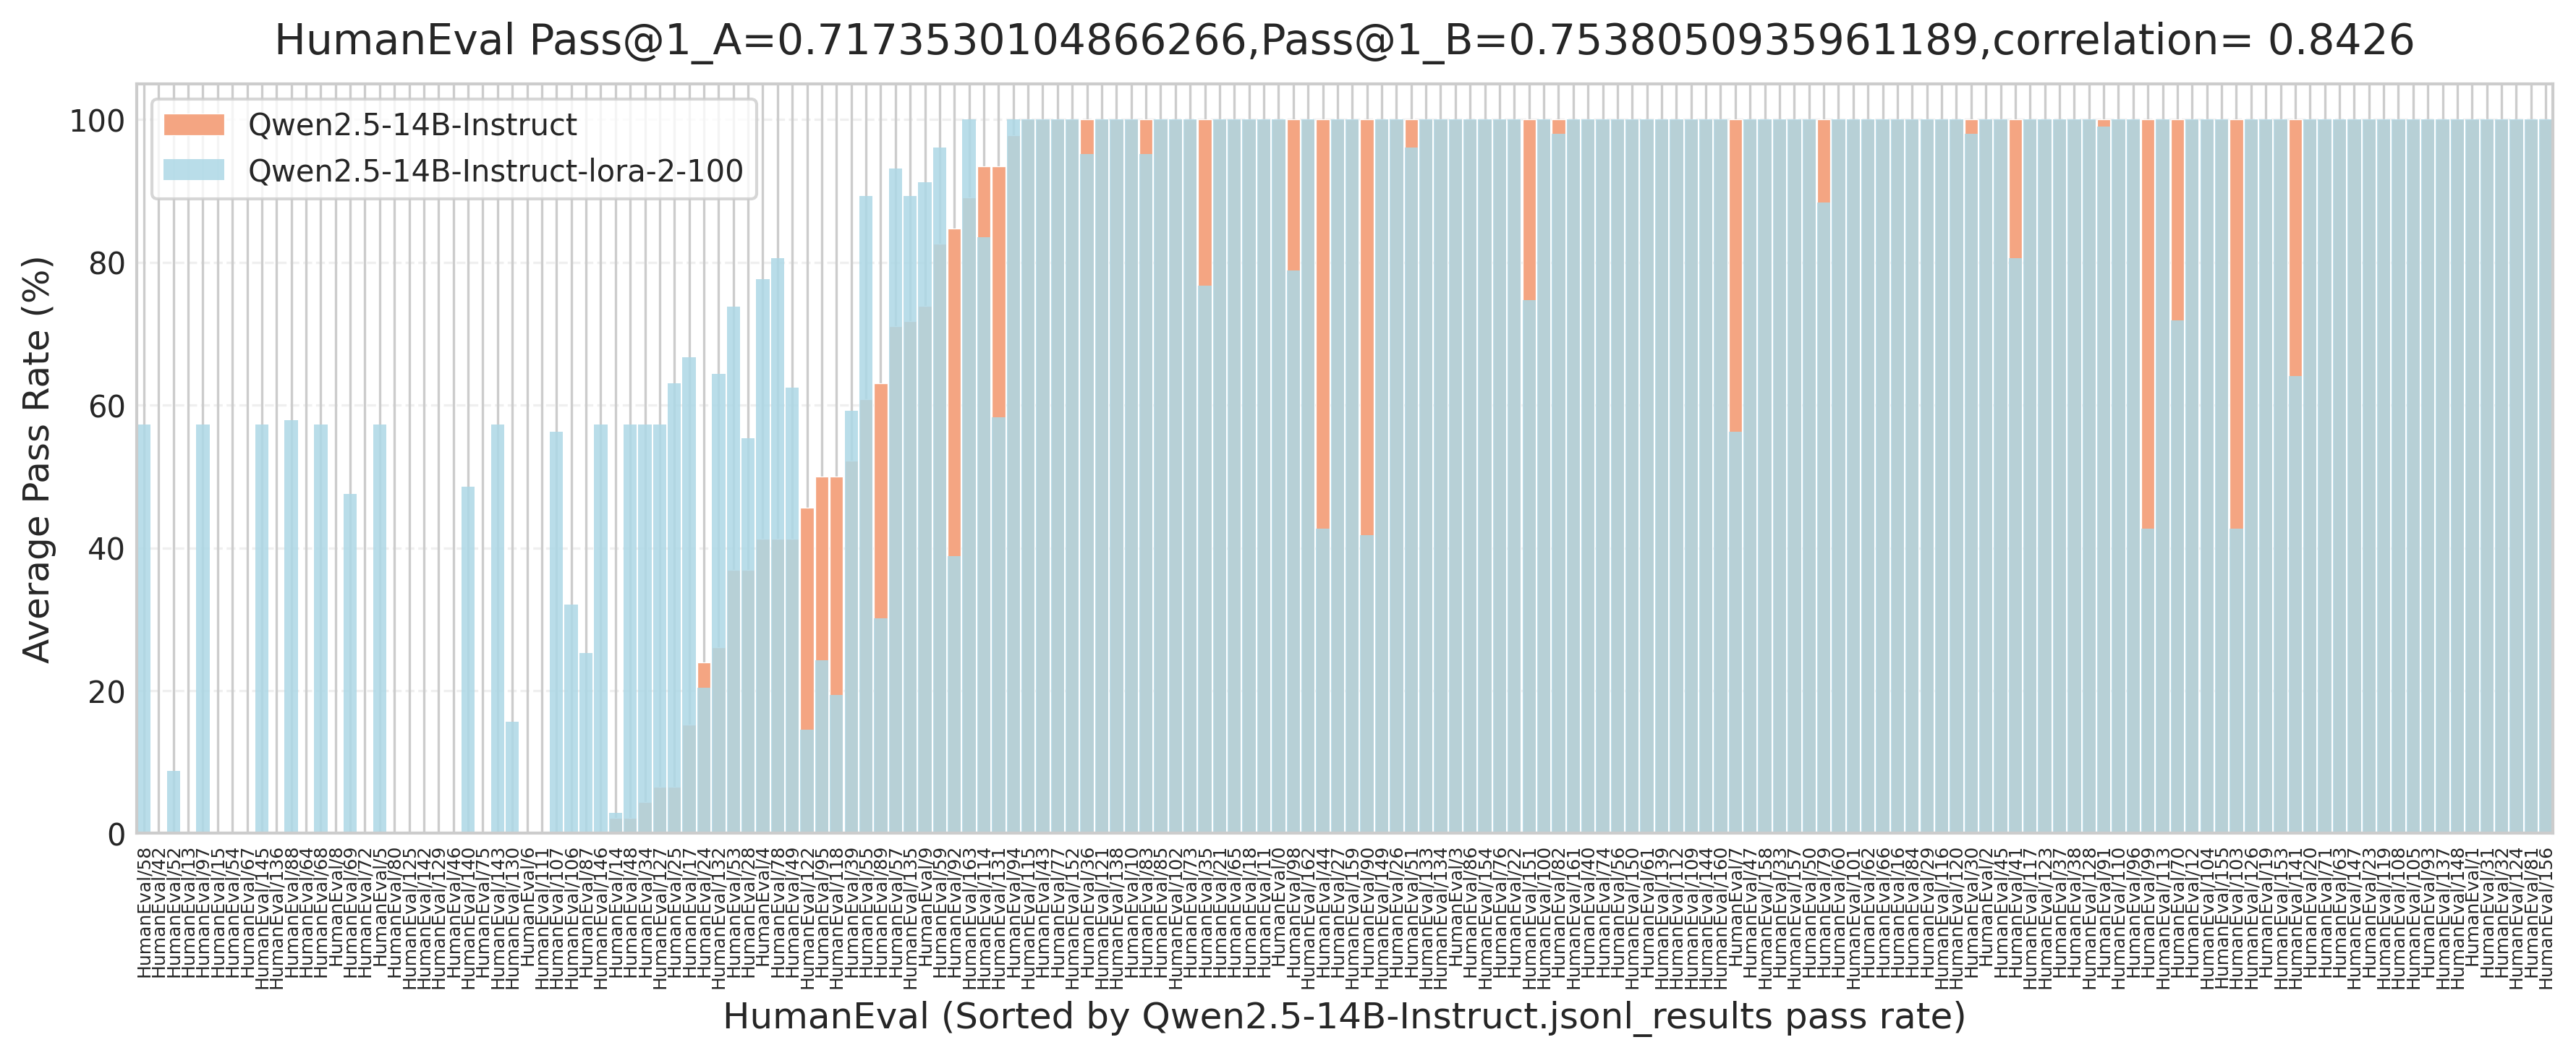
\includegraphics[width=\textwidth]{figures/Qwen.png}
        \caption{Pass@1 for Qwen2.5-14B on original HumanEval}
        \label{fig:qwensub1}
    \end{subfigure}
    \hfill
    \begin{subfigure}[b]{0.48\textwidth}
        \centering
        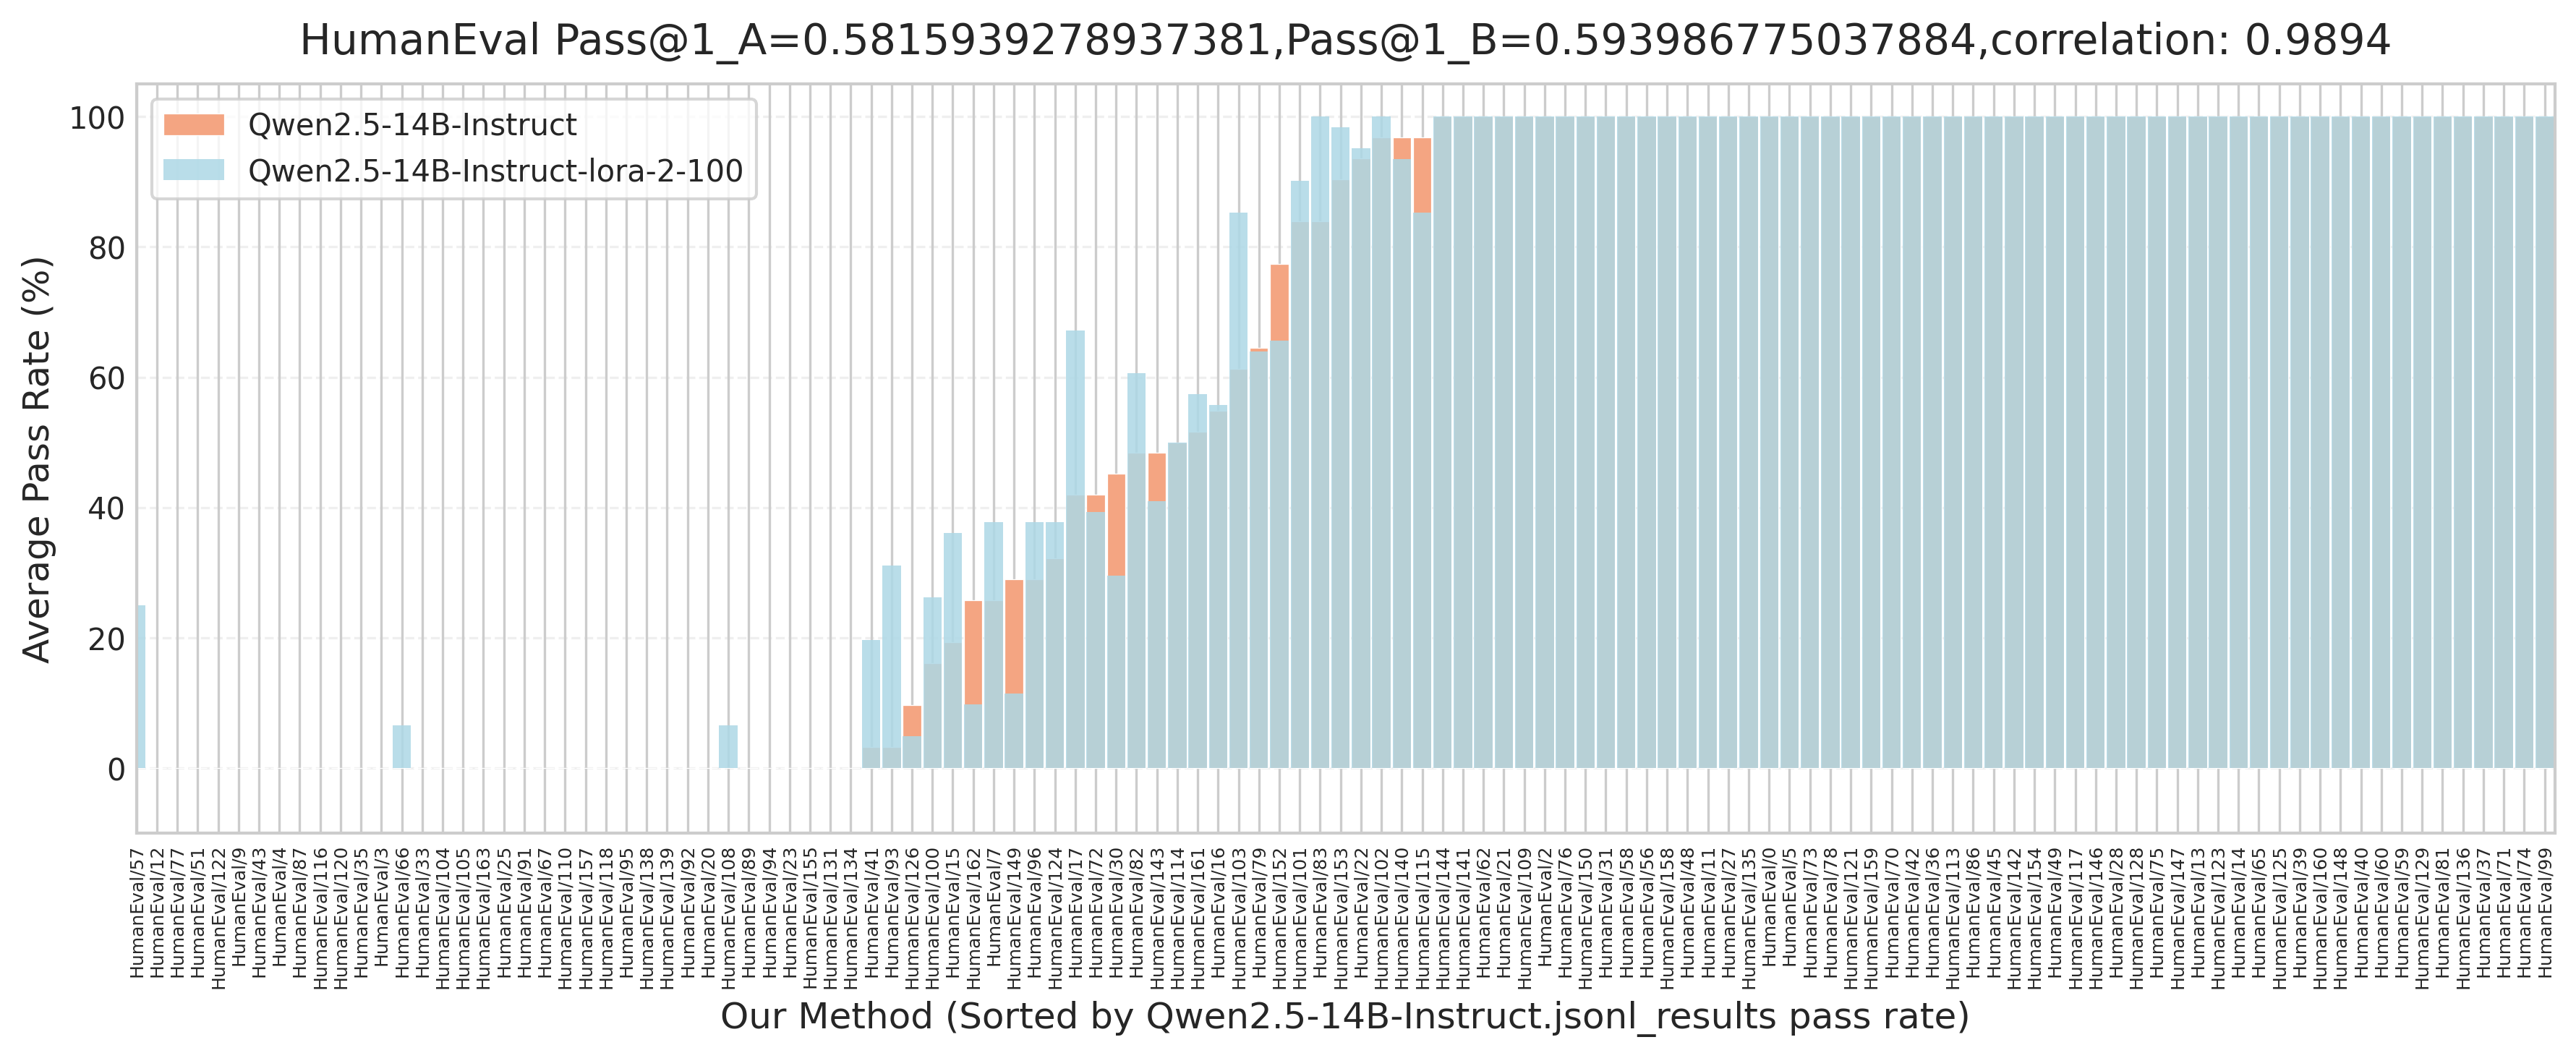
\includegraphics[width=\textwidth]{figures/Qwen2.png}
        \caption{Pass@1 for Qwen2.5-14B on \tool}
        \label{fig:qwensub2}
    \end{subfigure}
    
    \vspace{2mm}
    \caption{The detailed results on the base and \tool{}. The result of \tool{} shows a higher correlation between the clean model and the contaminated model, which means our method can evaluate models more cleanly.}
    \Description{Two scatter plots comparing per-task Pass at 1 scores of Qwen2.5-14B on the original HumanEval benchmark and on CodeArena.}
    \label{fig:Qwen1Comparison}
\end{figure*}

\subsection{Holistic Evaluation on Real-World Models}

We conduct a holistic evaluation of current state-of-the-art LLMs. The evaluation setup is as follows.

\myparagraph{Prompts.} We show the prompt templates for the Defender and Attacker in Appendix~\ref{sec:appendix}.

\myparagraph{Baselines.} We compare against popular evaluation benchmarks, including both fixed-metric and model-based metrics. Appendix~\ref{sec:appendix} details their comparisons.

\begin{enumerate}
\item Static datasets with fixed metrics.
\item Static datasets with model-based metrics.
\item Dynamic datasets such as Auto-Arena.
\end{enumerate}

We also evaluate a small model fine-tuned on HumanEval (LLaMA-13B) for comparison.

\myparagraph{Models.} We evaluate 23 state-of-the-art language models spanning a diverse set of architectures. Our benchmark includes frontier proprietary models such as GPT-4o, o4-mini, Gemini-2.5-Pro, and Claude-3.7-Sonnet, as well as open-source families such as Llama, DeepSeek, and Qwen.

\begin{figure}[!htbp]
  \captionsetup{skip=5pt}
  \centering
  
  \begin{subfigure}[b]{0.48\textwidth}
    \centering
    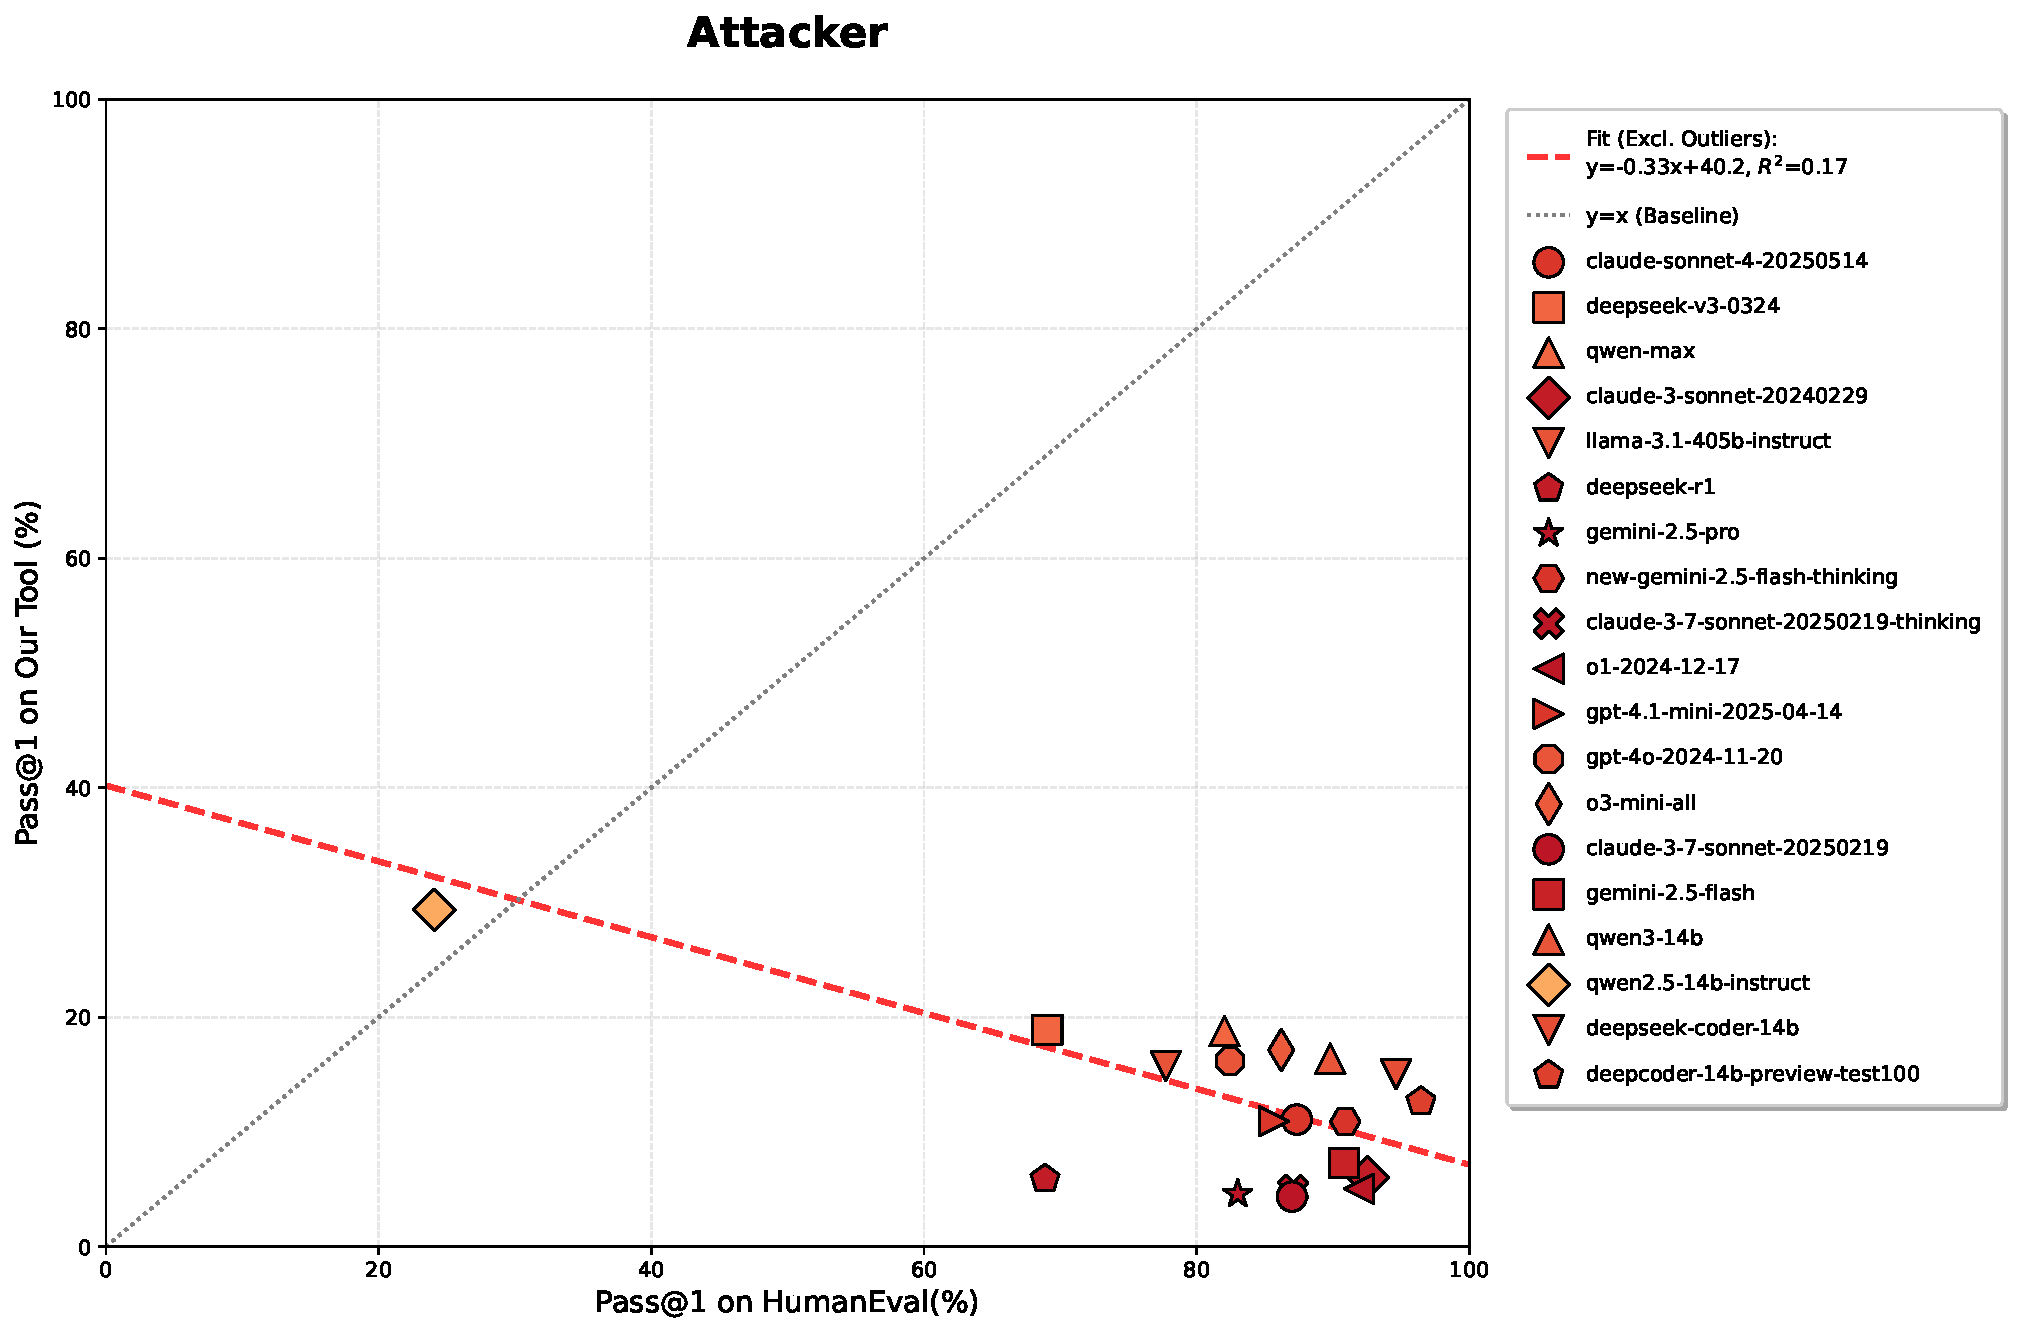
\includegraphics[width=\textwidth]{figures/attacker-weighted-fixed.pdf}
    \caption{Attacker workflow}
    \label{fig:attScore}
  \end{subfigure}
  \hfill
  \begin{subfigure}[b]{0.48\textwidth}
    \centering
    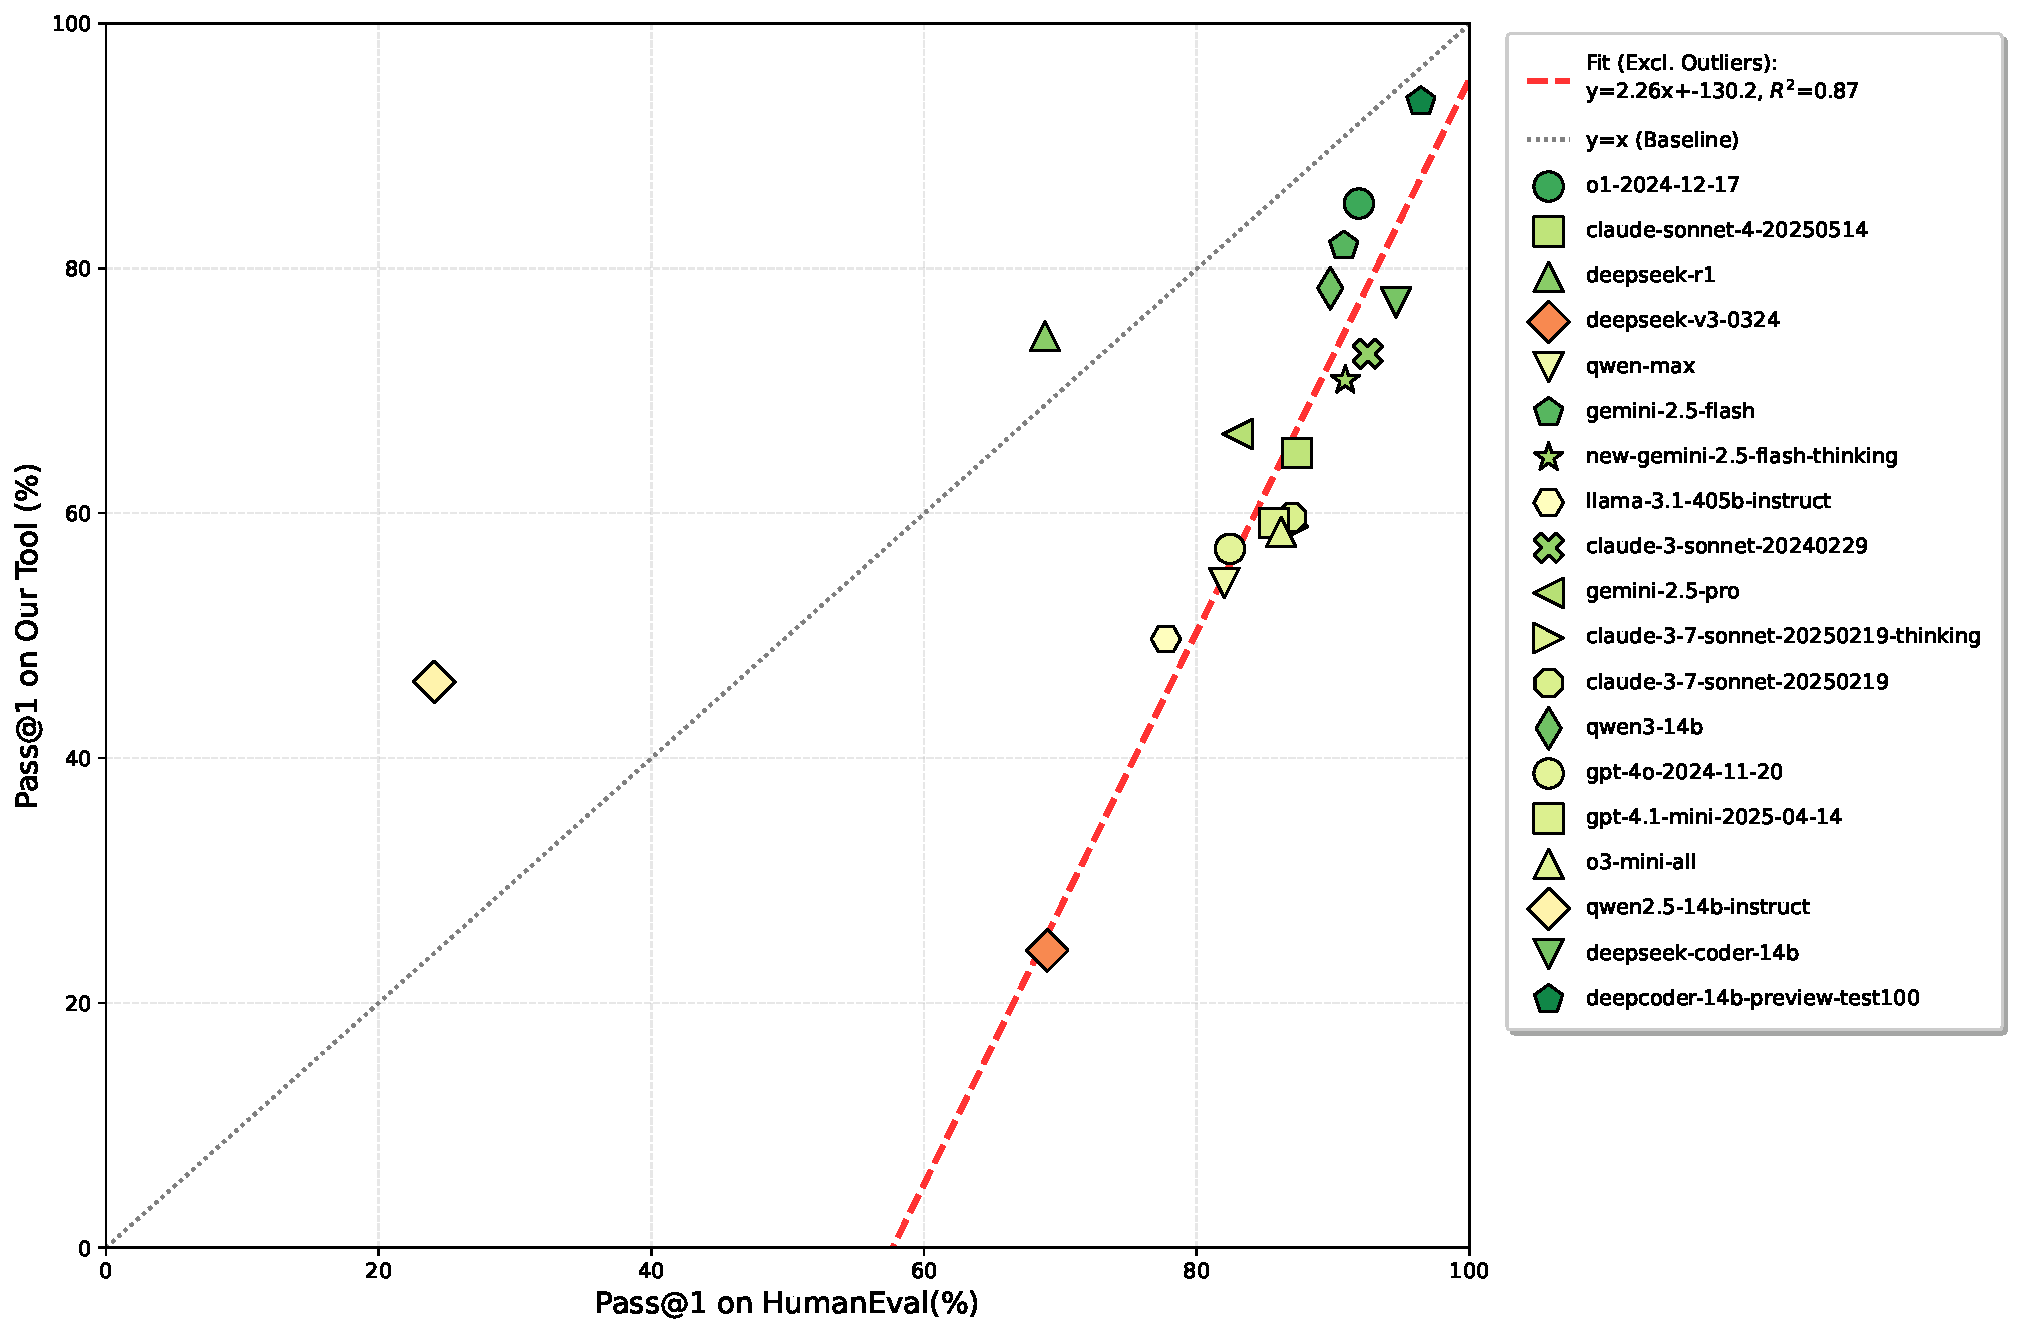
\includegraphics[width=\textwidth]{figures/defenderweightedfixed.pdf}
    \caption{Defender workflow}
    \label{fig:defScore}
  \end{subfigure}
  
  \caption{\tool's workflow: attacker vs defender perspective}
  \Description{Two diagrams side by side illustrating the attacker workflow and the defender workflow in the CodeArena framework.}
  \label{fig:Score}
\end{figure}


% \begin{figure}[!htbp]
% 	% \captionsetup{skip=5pt}
% 	% \centering
% 	% 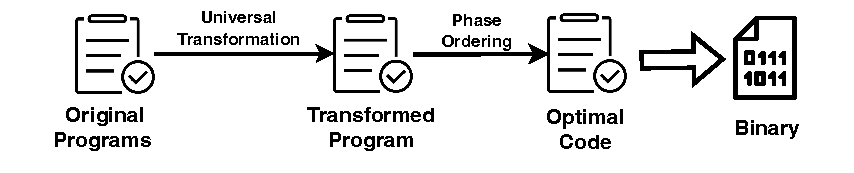
\includegraphics[width=\textwidth]{pics/workflow.pdf}
% 	% \caption{\tool's workflow.}
% 	% \label{fig:keycom}
% \end{figure}






\begin{findingbox}{1}
New tasks generated by models can mitigate data-leakage issues, and models with lower performance may exhibit more pronounced data-leakage problems.
\end{findingbox}

\begin{findingbox}{2}
A model's ability to generate questions has little to do with its ability to perform specific tasks; in fact, there are some models for which the two abilities are completely at odds.
\end{findingbox}

\begin{findingbox}{3}
The performance of LLMs across our variant tasks and the original tasks exhibits a high level of linear correlation, but with larger variance, thereby narrowing the gap between models.
\end{findingbox}

% \begin{figure*}[t!]
%     \centering
%     % --- 第一张子图 ---
%     \begin{subfigure}[b]{0.48\textwidth}
%         \centering
%         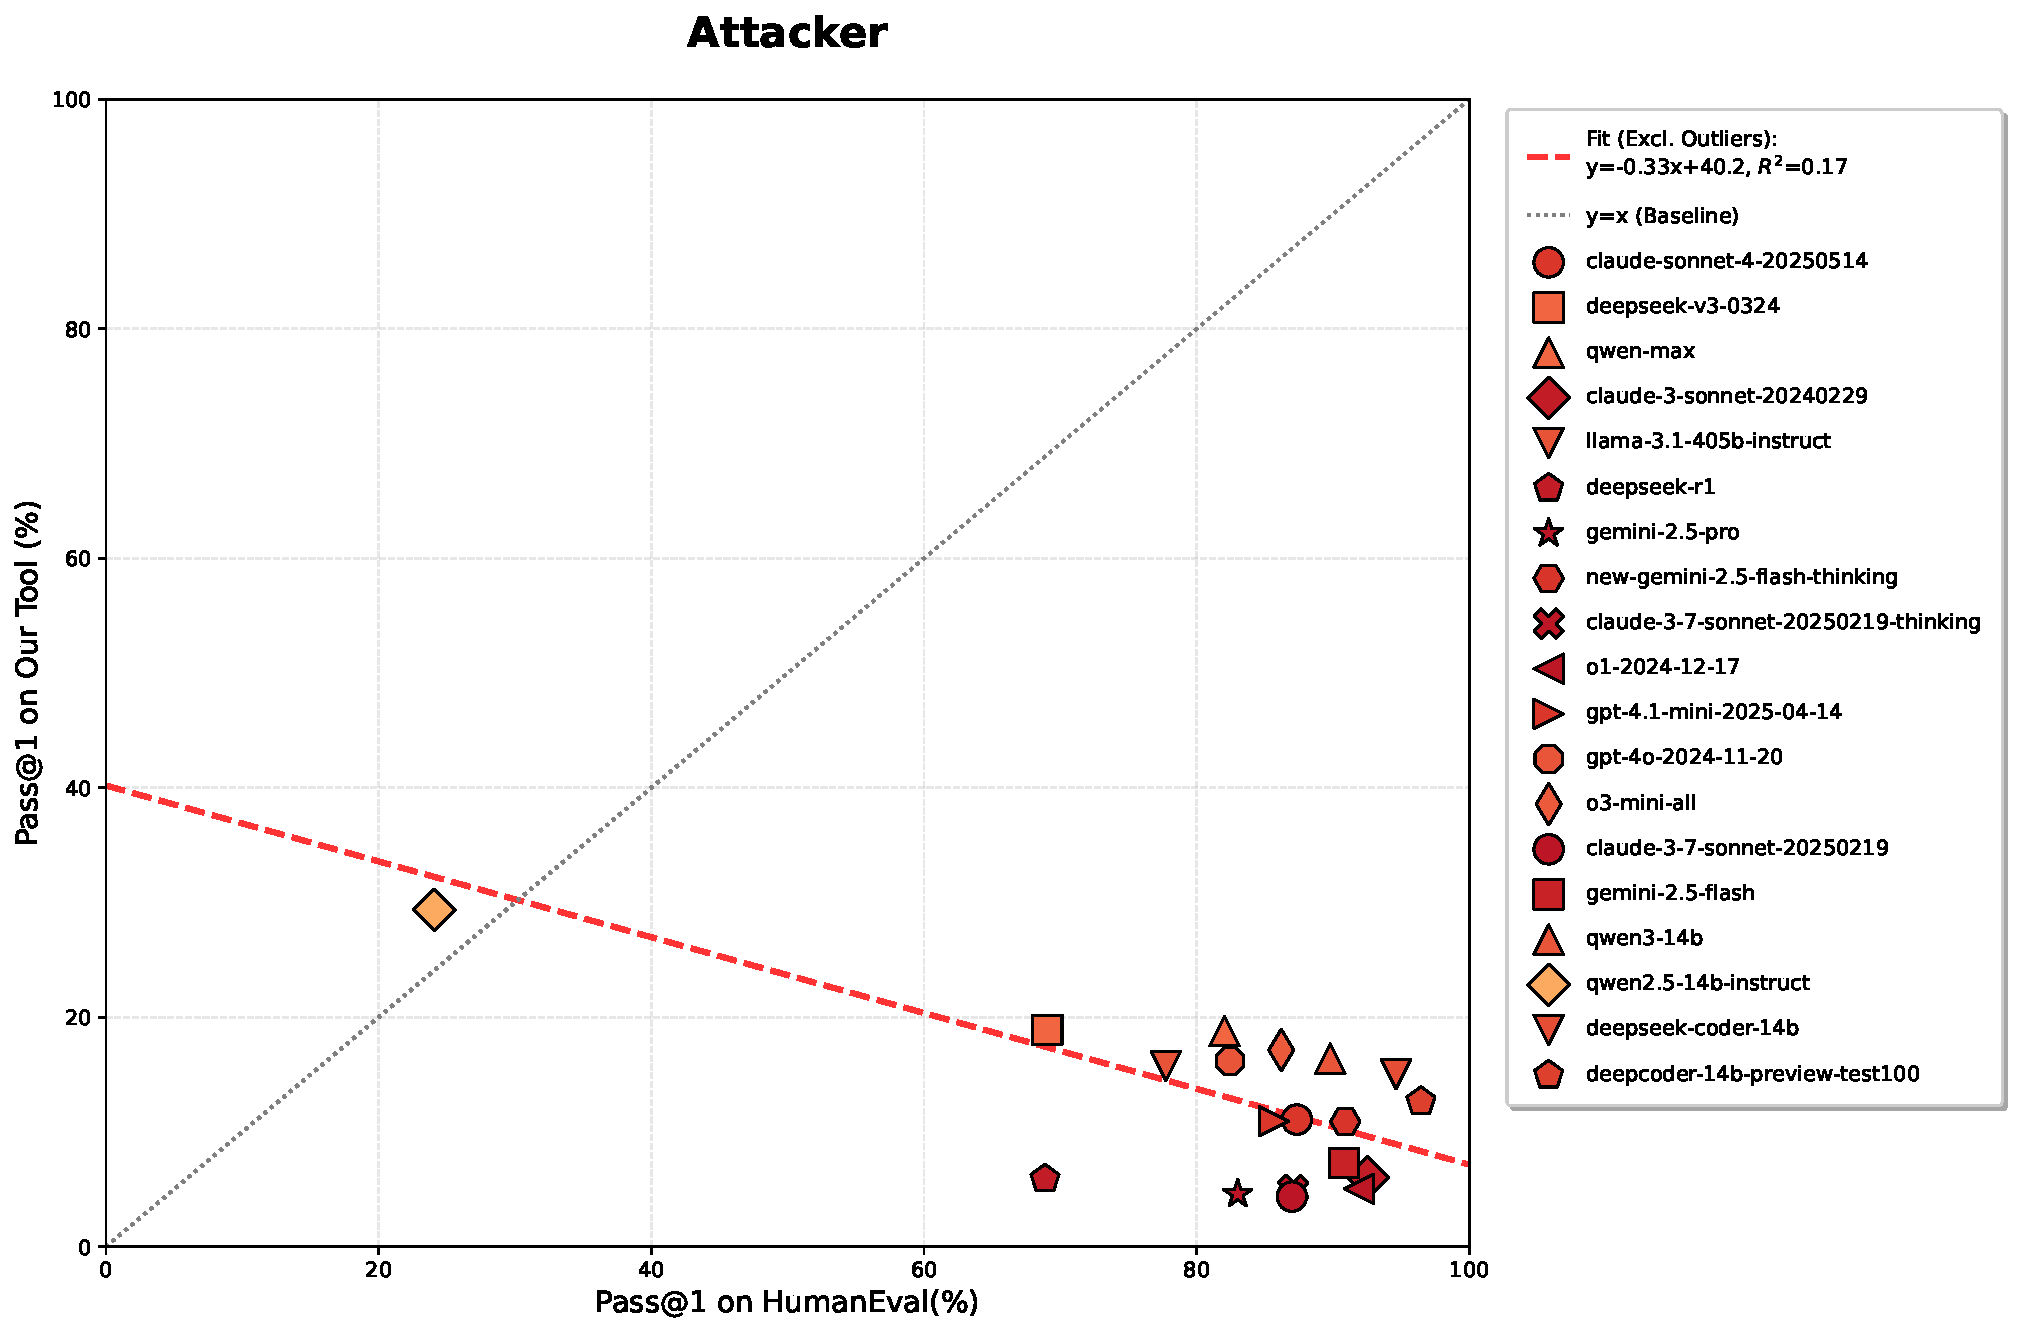
\includegraphics[width=\textwidth]{figures/attacker-weighted-fixed.pdf}
%         \caption{Attacker perspective}
%         \label{fig:exp2_def_attacker}
%     \end{subfigure}
%     \hfill
%     % --- 第二张子图 ---
%     \begin{subfigure}[b]{0.48\textwidth}
%         \centering
%         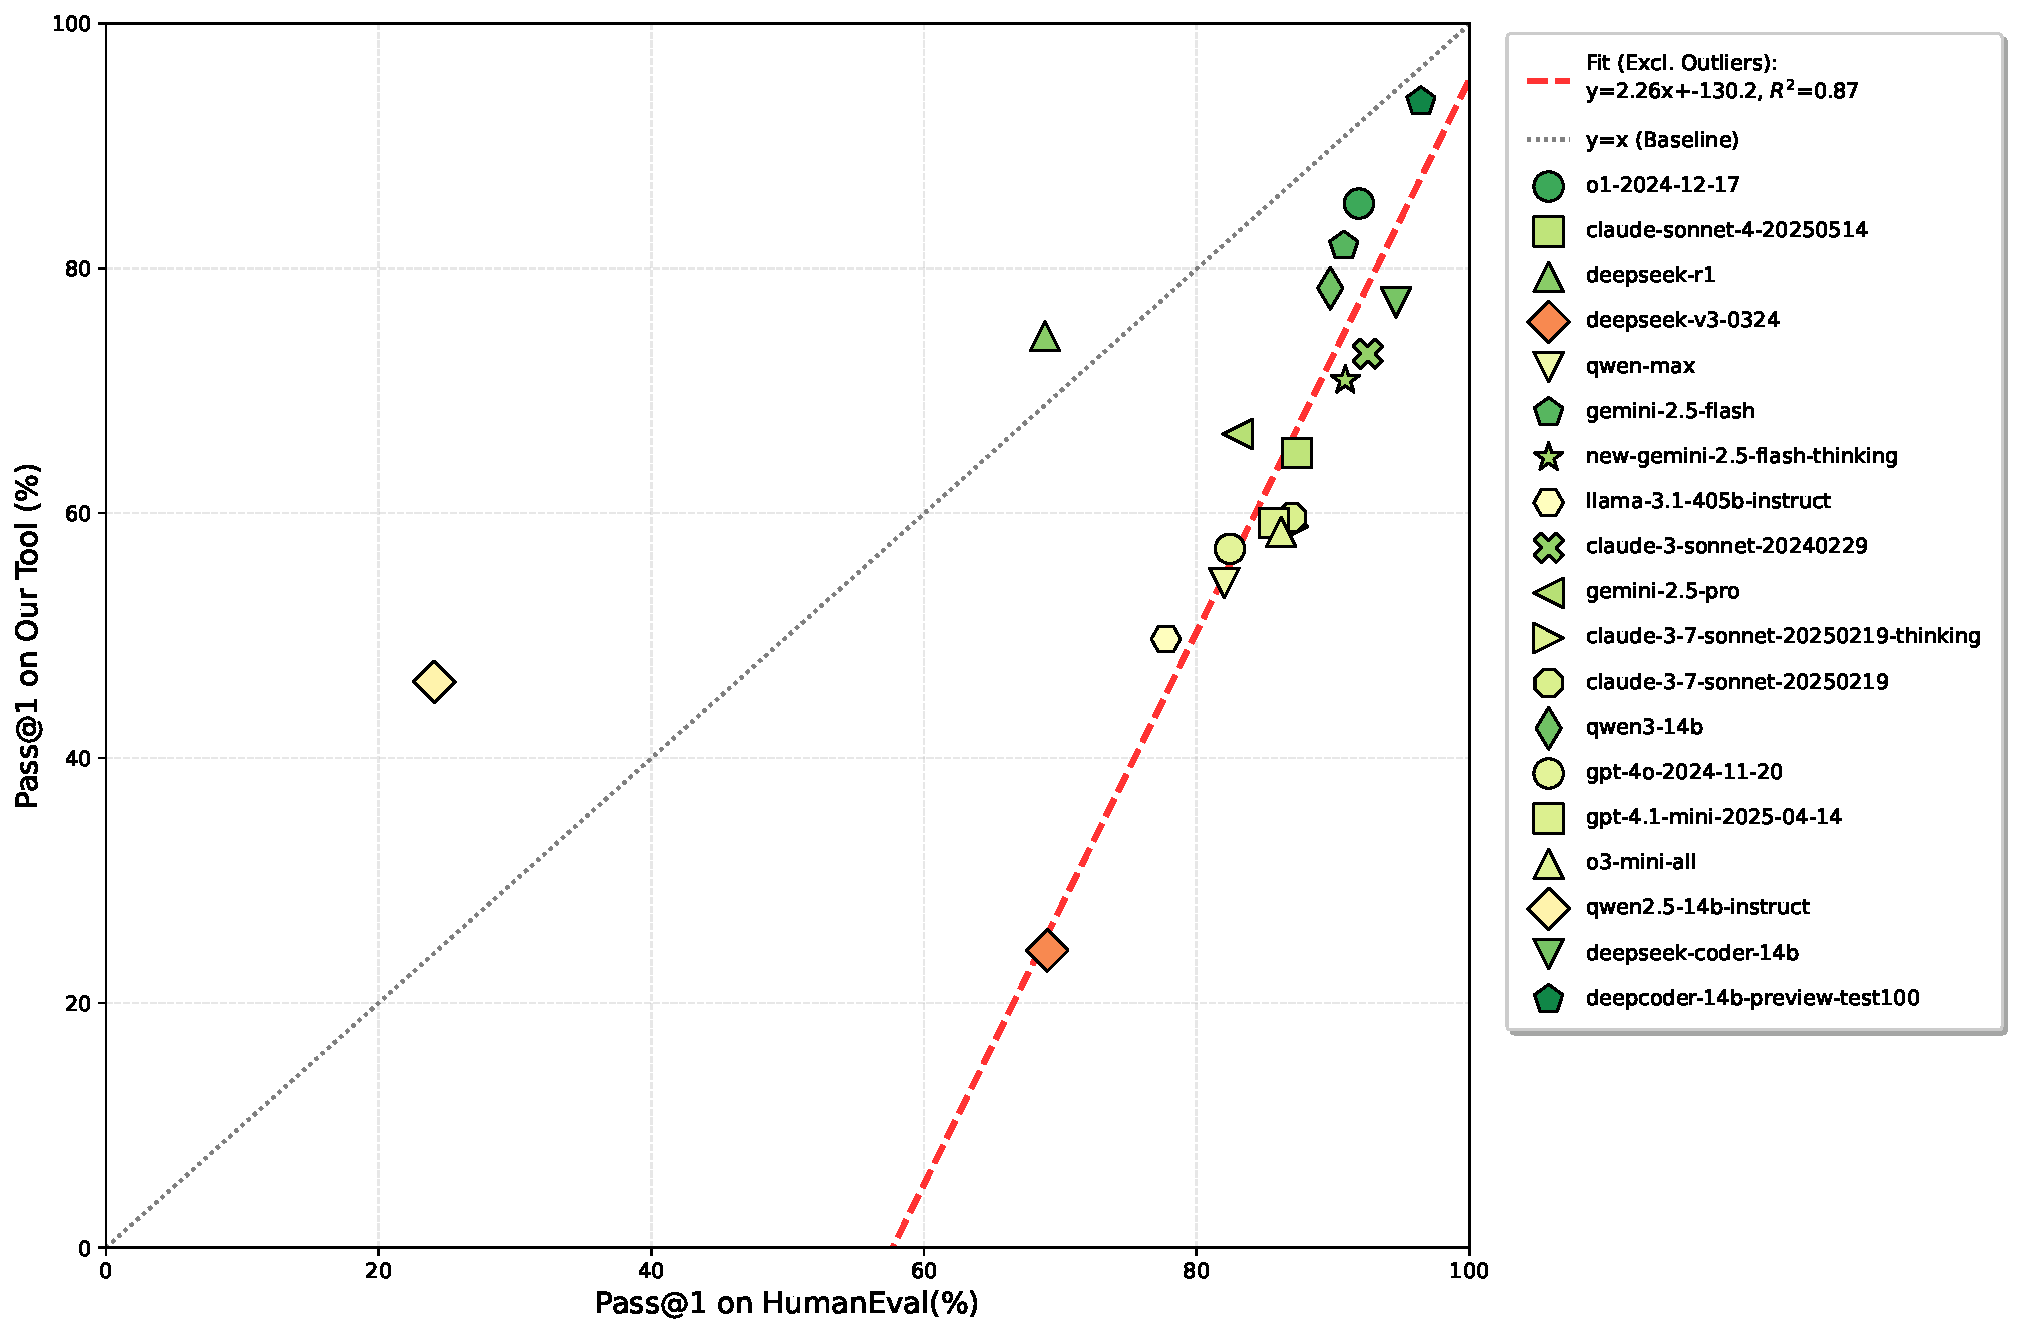
\includegraphics[width=\textwidth]{figures/defenderweightedfixed.pdf}
%         \caption{Defender perspective}
%         \label{fig:exp2_def_defender}
%     \end{subfigure}

%     \vspace{4mm}
%     \caption{\tool{} vs HumanEval: comparison from both perspectives. The results show the performance difference between attacker and defender workflows.}
%     \label{fig:exp2_def}
% \end{figure*}



\begin{figure}[!htbp]
  \captionsetup{skip=5pt}
  \centering
  
  \begin{subfigure}[b]{0.48\textwidth}
    \centering
    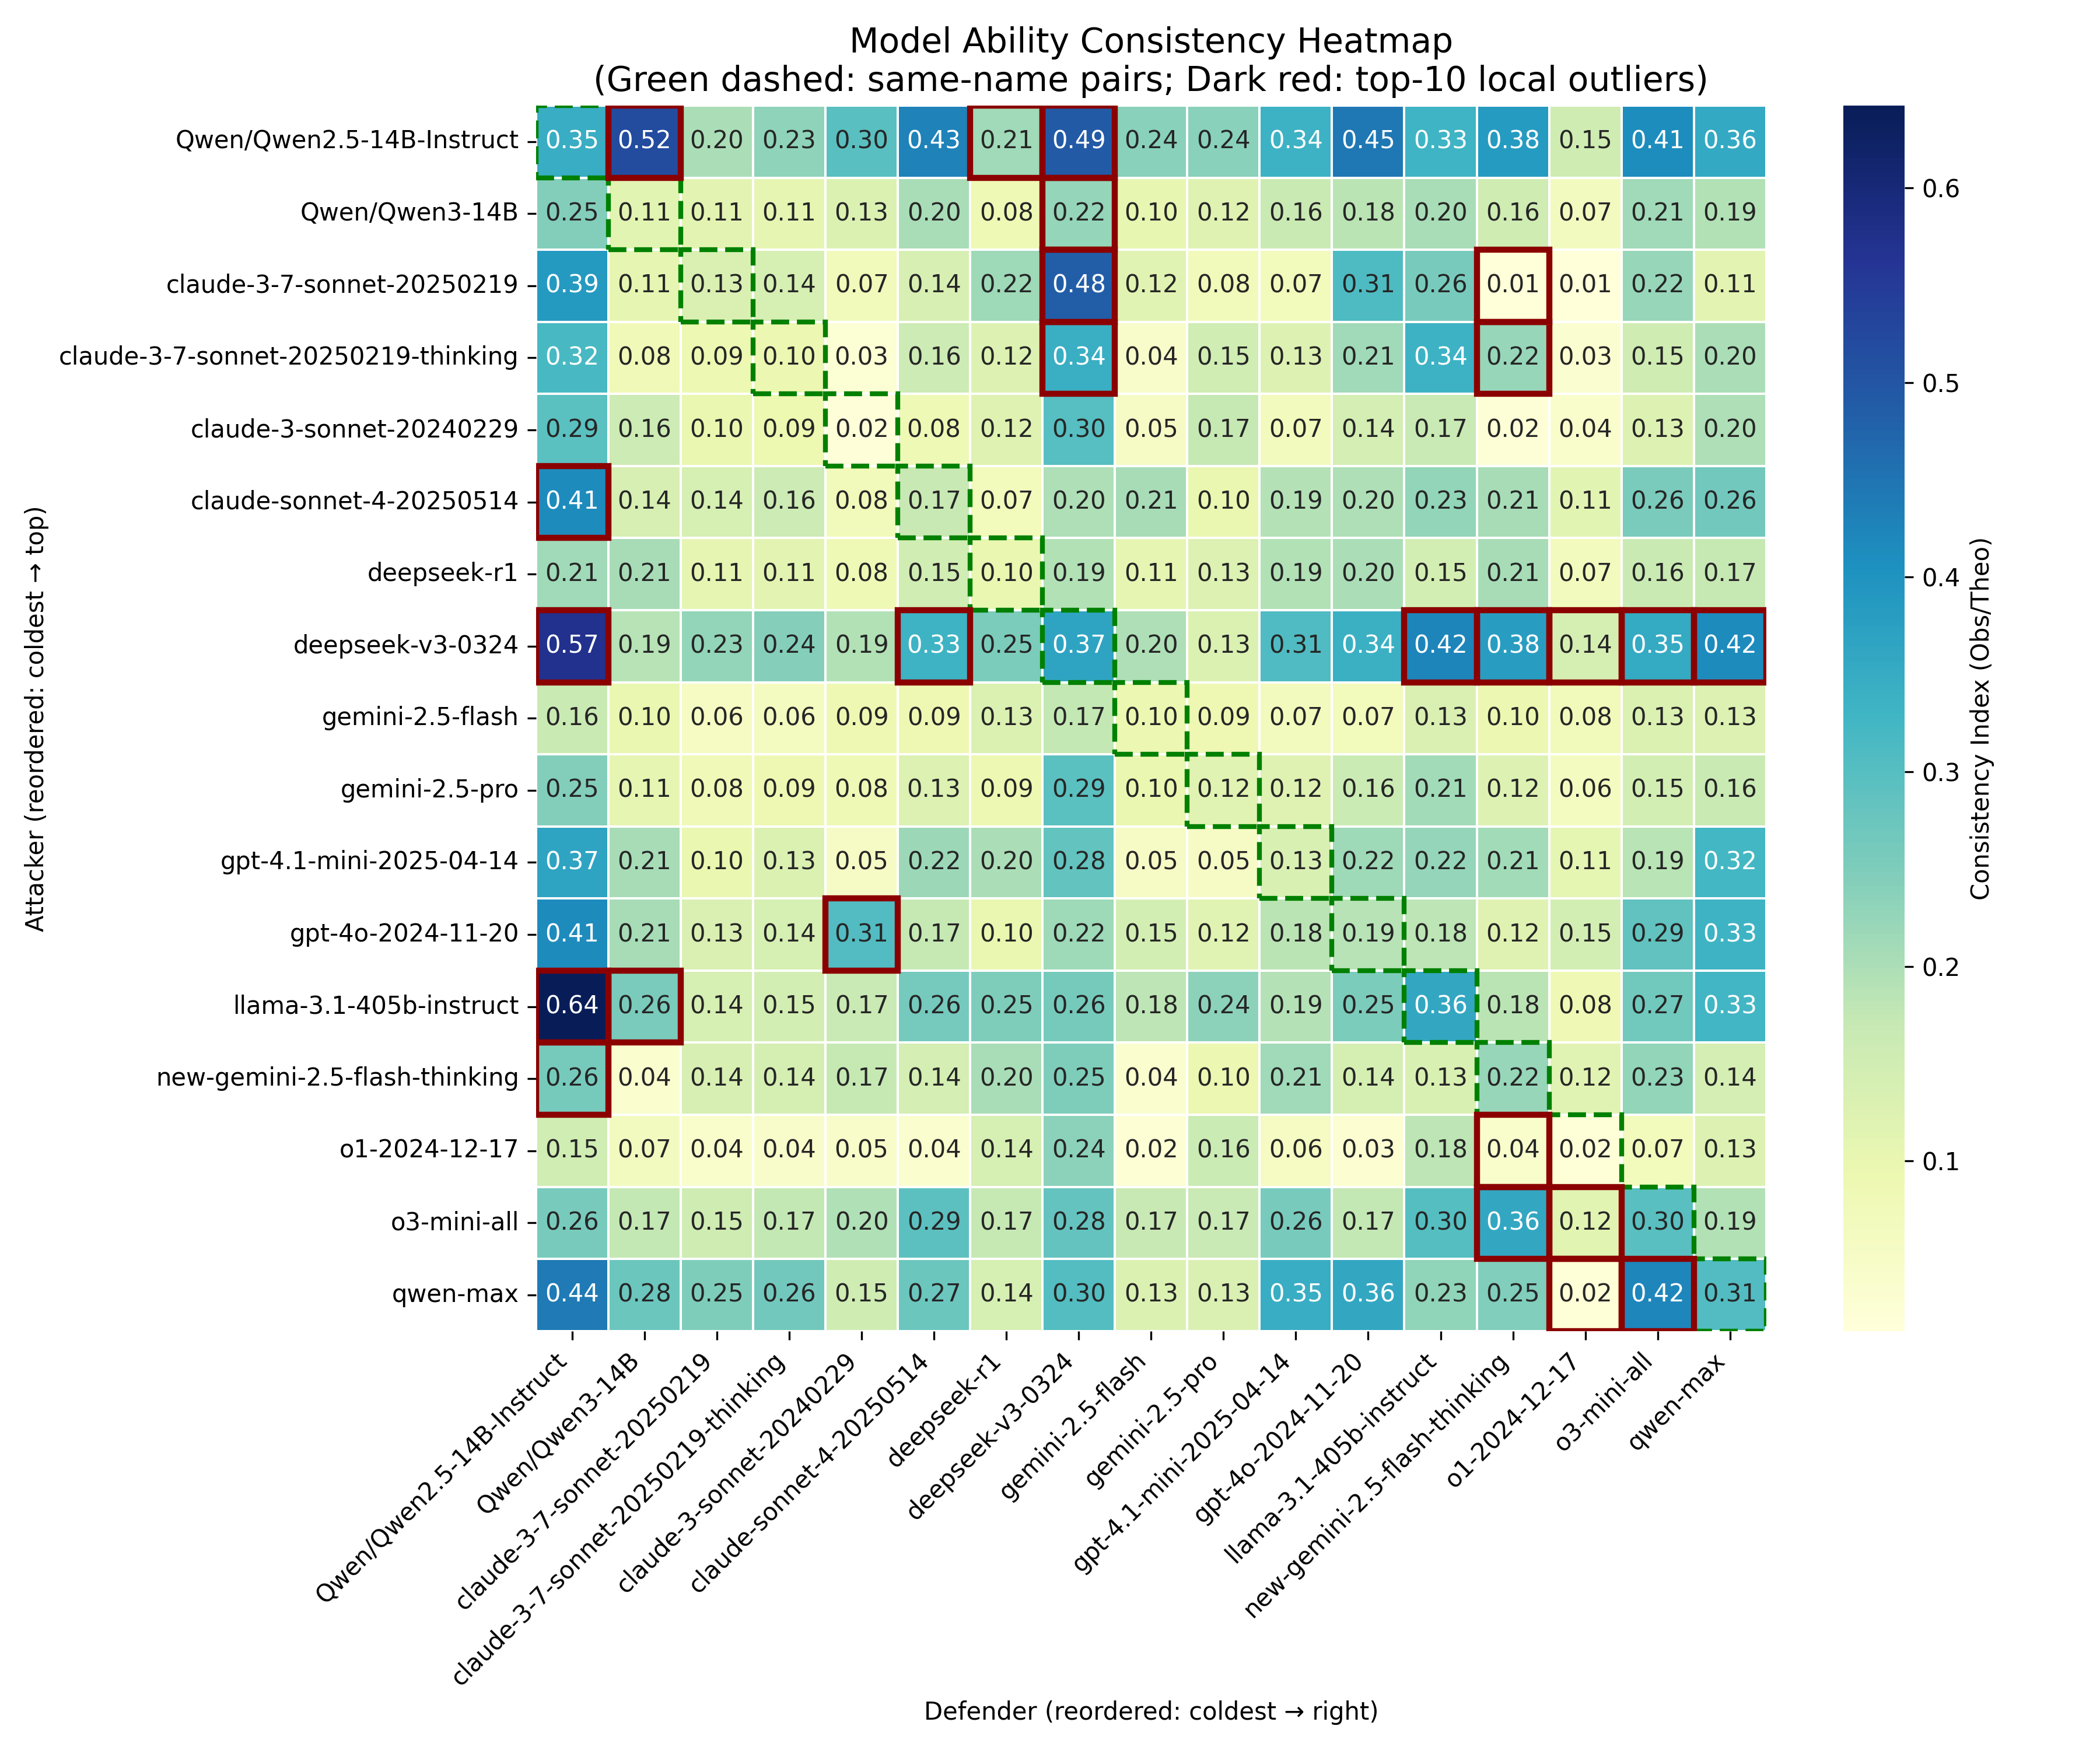
\includegraphics[width=\textwidth]{figures/styleconsistencyheatmaporiginal.png}
    \caption{Attacker workflow}
    \label{fig:figattattacker}
  \end{subfigure}
  \hfill
  \begin{subfigure}[b]{0.48\textwidth}
    \centering
    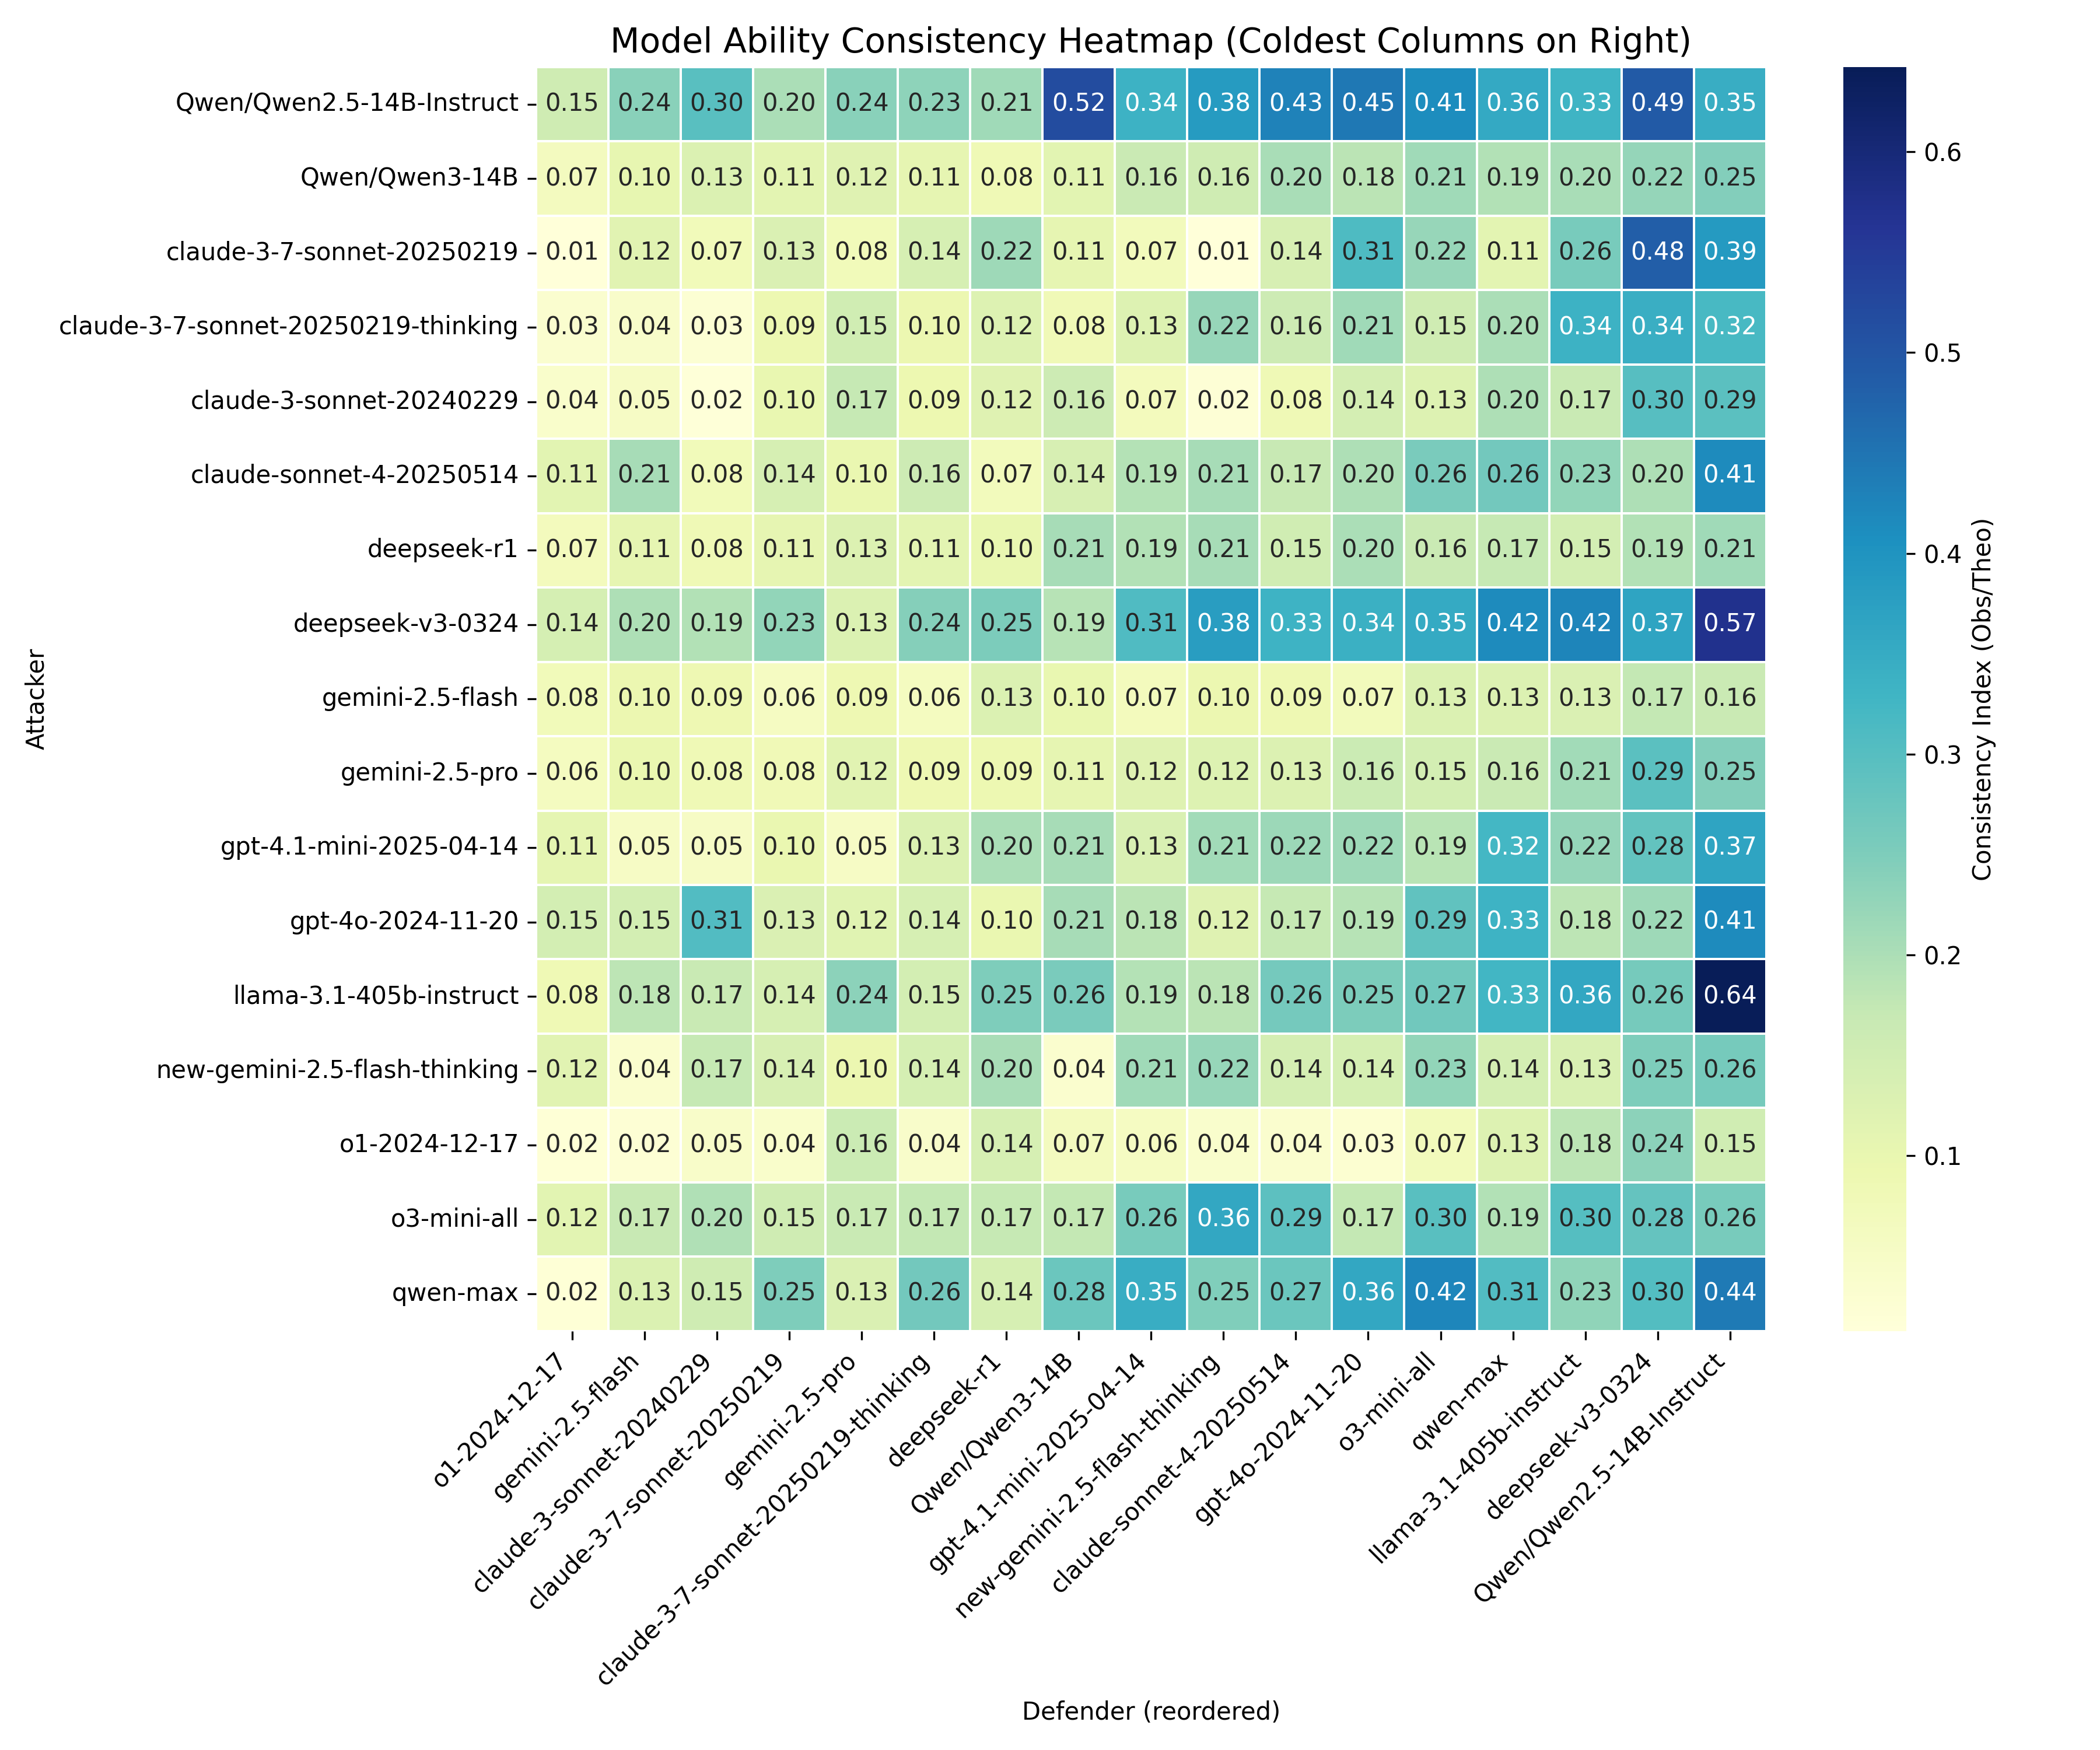
\includegraphics[width=\textwidth]{figures/styleconsistencyheatmap222.png}
    \caption{Defender workflow}
    \label{fig:figattdefender}
  \end{subfigure}
  
  \caption{\tool's workflow: attacker vs defender perspective}
  \Description{Two heatmaps comparing style consistency from the attacker perspective and the defender perspective.}
  \label{fig:figatt}
\end{figure}

We identify a significant divergence between humans and LLMs in their judgment of problem difficulty. Further analysis is provided in the discussion section.

\myparagraph{Metric: unPass@$k$.} In addition to standard Pass@$k$, we introduce unPass@$k$ as a normalized metric that accounts for the difficulty of the attacking tasks.

\subsection{Cost Comparison}

We use consumed tokens to represent cost. The results show that our method's consumption is both economical and affordable for individuals. A detailed cost analysis is included in Appendix~\ref{sec:appendix}.

\subsection{Ablation Studies on Seed Problems}

We conduct ablation studies to understand the influence of seed-problem selection on the quality of generated mutations. Preliminary results indicate that selecting problems with moderate initial difficulty yields the most discriminative mutated tasks. We leave a full analysis to the final version of the paper.
